

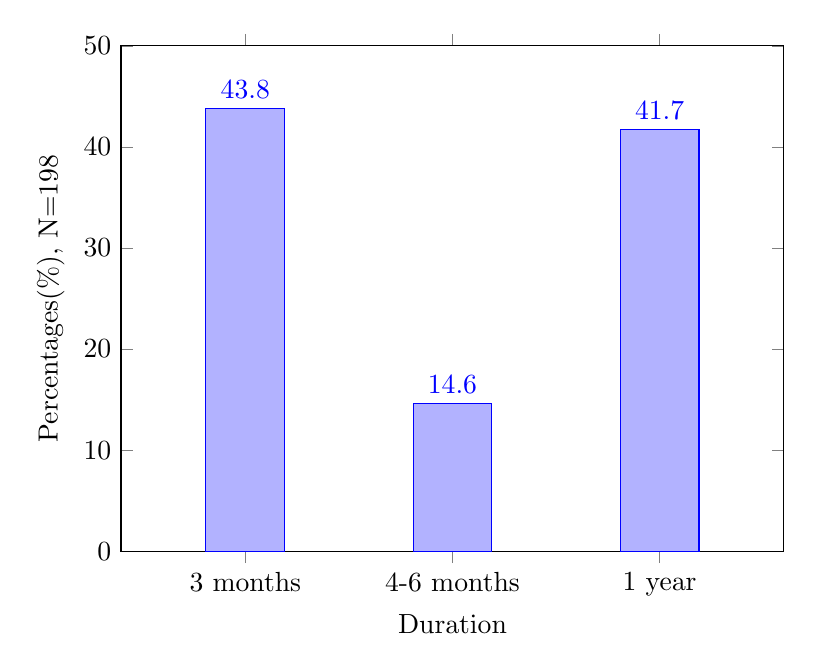
\begin{tikzpicture}
\begin{axis}[
    ybar,
    bar width=1cm,
    width=10cm, % Adjust the width to fit your needs
    height=8cm, % Adjust the height to fit your needs
    xlabel={Duration},
    ylabel={Percentages(\%), N=198},
    symbolic x coords={3 months, 4-6 months, 1 year},
    xtick=data,
    nodes near coords,
    nodes near coords align={vertical},
    ymin=0, % Start y-axis from 0
    ymax=50, % Set the maximum value of y-axis
    enlarge x limits=0.3, % Add some space around the bars
]

\addplot coordinates {(3 months,43.8) (4-6 months,14.6) (1 year,41.7)};

\end{axis}
\end{tikzpicture}

